\documentclass[12pt, letterpaper]{article}
%\setlength{\parindent}{0in}
\setlength{\textheight}{8.9in}
\setlength{\textwidth}{6.8in}
\setlength{\oddsidemargin}{-0.3in}
\setlength{\evensidemargin}{0.0in}
\addtolength{\topmargin}{-1in}
\setlength{\parskip}{0.1in}

\usepackage{amsmath, amsfonts}
\usepackage{graphicx}
\usepackage{setspace}
\usepackage{color}
\onehalfspacing

\newcommand{\bmeta}{\boldsymbol{\eta}}
\newcommand{\bmtheta}{\boldsymbol{\theta}}
\newcommand{\bmbeta}{\boldsymbol{\beta}}
\newcommand{\bmphi}{\boldsymbol{\phi}}
\newcommand{\bmpi}{\boldsymbol{\pi}}
\newcommand{\bmxi}{\boldsymbol{\xi}}
\newcommand{\bmnu}{\boldsymbol{\nu}}
\newcommand{\bmmu}{\boldsymbol{\mu}}
\newcommand{\bmalpha}{\boldsymbol{\alpha}}
\newcommand{\bmzeta}{\boldsymbol{\zeta}}
\newcommand{\bmgamma}{\boldsymbol{\gamma}}

\newcommand{\bmY}{\mathbf{Y}}
\newcommand{\bmZ}{\mathbf{Z}}
\newcommand{\bmX}{\mathbf{X}}
\newcommand{\bmV}{\mathbf{V}}
\newcommand{\bmW}{\mathbf{W}}
\newcommand{\bmR}{\mathbf{R}}
\newcommand{\bmS}{\mathbf{S}}
\newcommand{\bmb}{\mathbf{b}}

\newcommand{\bmM}{\mathbf{M}}
\newcommand{\bmSigma}{\boldsymbol{\Sigma}}
\newcommand{\bmI}{\mathbf{I}}
\newcommand{\bmTheta}{\boldsymbol{\Theta}}


\newcommand{\bea}{\begin{eqnarray}} 
\newcommand{\eea}{\end{eqnarray}} 
\newcommand{\beas}{\begin{eqnarray*}} 
\newcommand{\eeas}{\end{eqnarray*}} 
\newcommand{\benum}{\begin{enumerate}} 
\newcommand{\eenum}{\end{enumerate}} 
\newcommand{\bd}{\begin{description}}
\newcommand{\ed}{\end{description}}
\newcommand{\bi}{\begin{itemize}}
\newcommand{\ei}{\end{itemize}}

\definecolor{mygreen}{rgb}{0,0.75,0}
\definecolor{mypurple}{rgb}{0.7,0,0.8}

\newcommand{\highlight}[1]{\colorbox{yellow}{#1}}
\newcommand{\gbox}[1]{\colorbox{green}{#1}}
\newcommand{\tcr}[1]{\textcolor{red}{#1}}
\newcommand{\tcg}[1]{\textcolor{mygreen}{#1}}
\newcommand{\tcb}[1]{\textcolor{blue}{#1}}
\newcommand{\tcp}[1]{\textcolor{mypurple}{#1}}
\newcommand{\tcbk}[1]{\textcolor{black}{#1}}


\begin{document}

\begin{center}
\large Prediction Model for Active Surveillance of Prostate Cancer\\
Rebecca Yates Coley\\
March 27, 2015\\
\end{center}

\section{Introduction }

We have developed a Bayesian, joint hierarchical model that predicts the underlying cancer state, PSA trajectory, and future biopsy results for individuals in the Johns Hopkins Active Surveillance Cohort. 

\section{Model}



The DAG in Figure \ref{fig:pred-dag} illustrates the assumed relationships between variables. Blue circles are used to denote the perfect measurement of these variables, if they could be obtained, and green circles indicate observations of the variables of interest that are made with error. We describe latent and observed variables below, as well as the statistical models we use to investigate their relationships.

\begin{figure}[b*]
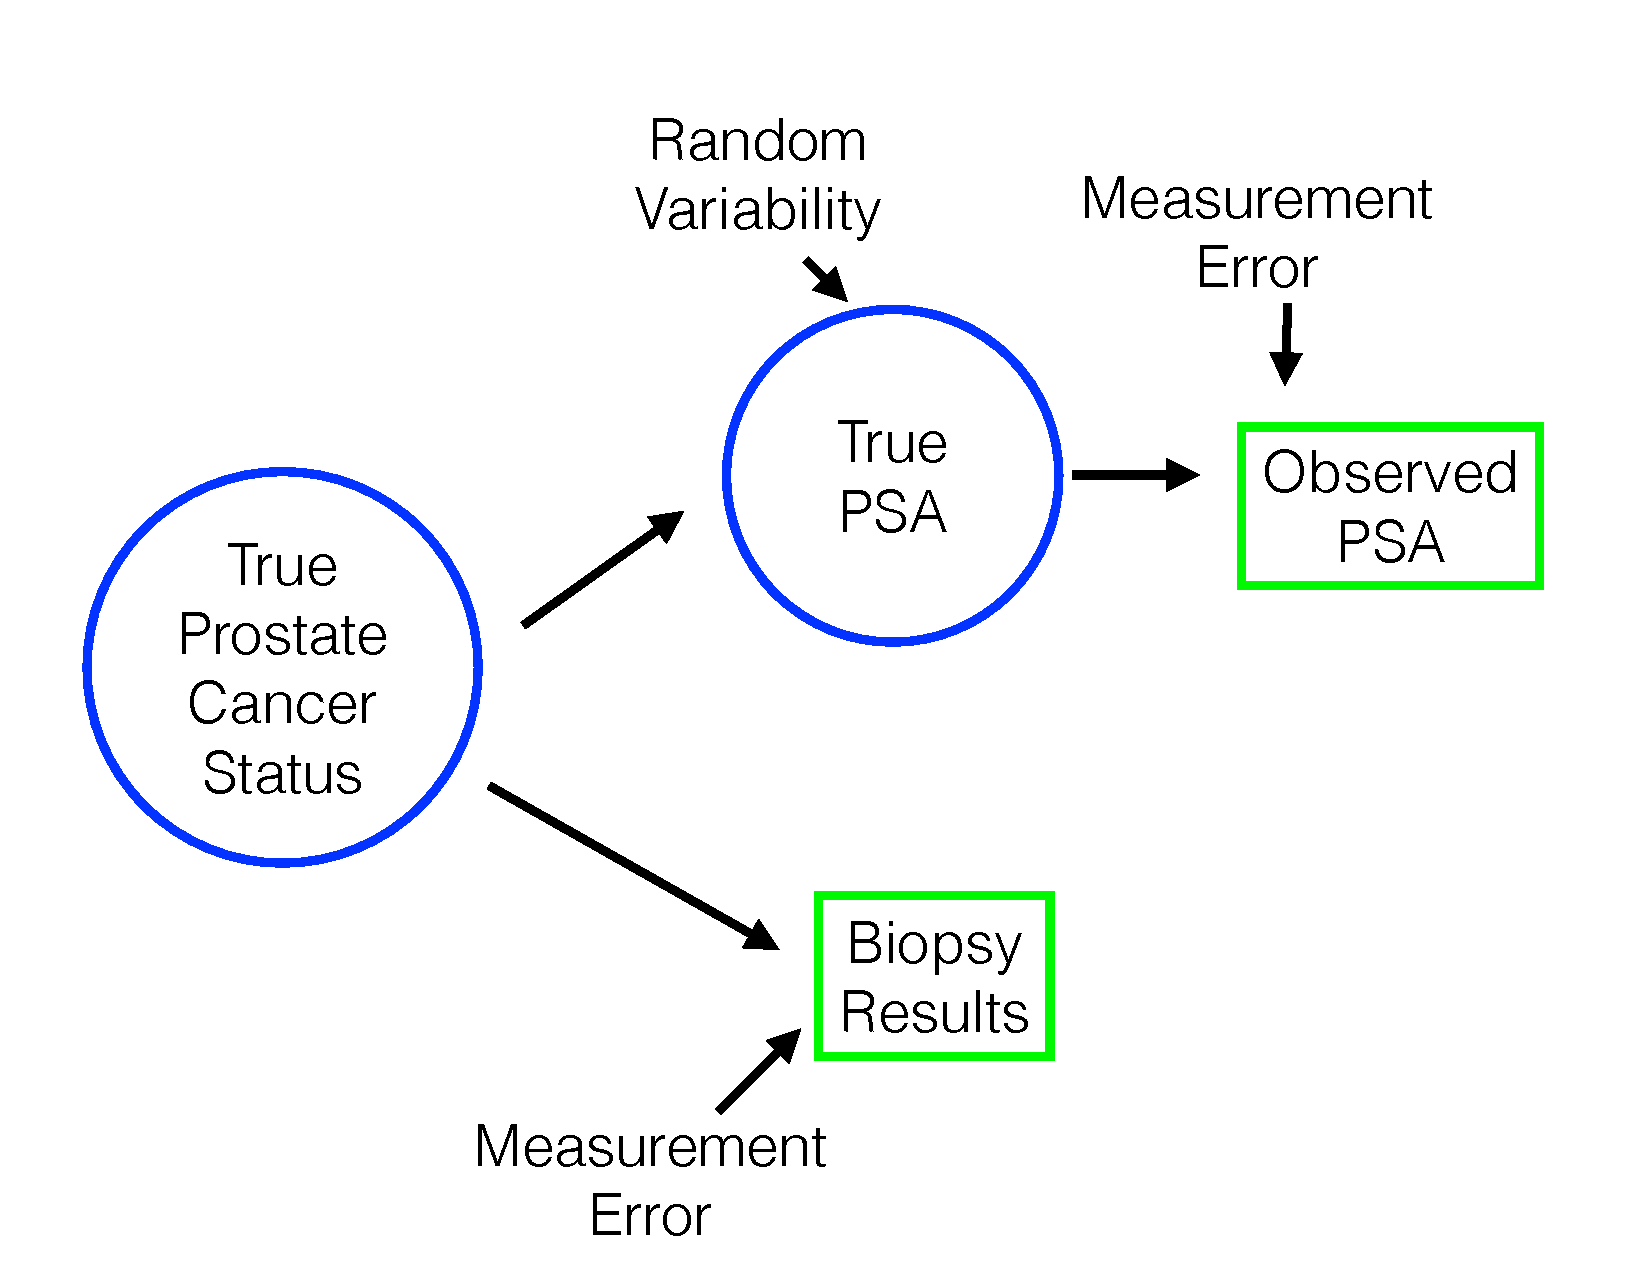
\includegraphics[scale=0.5]{pred-dag}
\caption{Directed acyclic graph}
\label{fig:pred-dag}
\end{figure}

\subsection{Latent Class Model}
We first define each man's underlying true cancer state as the prognostic grade score that would be assigned if the entire prostate were to be removed and a pathological analysis performed. Since we only observe this true cancer state on the subset of patients in active surveillance who choose surgical removal of the prostate (approximately 15$\%$), we model true cancer state as a partially observed latent variable, which we denote \highlight{$\eta_i$}. This definition assumes that there is no variability in grading for full prostate specimens and that all observed grade determinations are correct. It also assumes that an individual's prostate cancer state does not change over the time period under consideration. Under this conceptual framework, a prostate cancer is assumed to manifest its true state over time. More lethal cancers are considered fundamentally different from indolent ones from their inception and it is assumed the same histology would be observed if a full pathological analysis was performed earlier.  

For our initial model, we assume a binary latent cancer state: indolent (Gleason score 6 or prognostic grade group 1) or potentially lethal (Gleason score 7 or above or prognostic grade group 2-5), and denote these classes with $\eta=0$ and $\eta=1$, respectively. We do not use covariates to model latent cancer state; instead we assume a shared, underlying probability distribution for latent class membership, \highlight{$\rho$}, i.e. $P(\eta_i=1) = \rho$ for all individuals $i=1,\dots,n.$ 

\subsubsection{Regressions Models for Latent Cancer Status}
%\textit{Aaron- no need to get bogged down in the details in this subsection, but whatever method we choose will need to be able to update $\eta$ under a more complicated model. I introduce the model we will likely use below.}
\textit{In the current model, we aren't using models described in this subsection.}

The choice of model for latent cancer state depends on how many levels the variable takes and the assumed relationship between latent cancer state and baseline covariates. For a binary latent variable (i.e., insolvent vs. lethal), a logistic regression model is natural:
\beas
P(\eta_i=k | \bmV_i) = \text{logit}^{-1}\big(\bmV_i \bmnu\big) 
\eeas
Here, \highlight{$\bmV_i$} is a vector of baseline covariates for individual $i$ and \highlight{$\bmnu$} is a parameter vector modeling the association between $\bmV_i$ and $\eta_i$. (Since latent class is assumed to be constant over time, only baseline covariates are used.)

In the future, we may model latent cancer state as an ordinal variable corresponding to each prognostic grade group, i.e. $\eta_i \in (1,2,3,4,5)$. Modeling options are more numerous for an ordinal outcome variable, but we will likely use a cumulative link model:
\beas
G^{-1}\big(P(\eta_i \leq k | \bmV_i)\big) =  \alpha_k - \bmV_i\zeta_k
\eeas
where $\alpha_k$ is an intercept parameter satisfying $-\infty=\alpha_0<\alpha_1<\dots<\alpha_{k-1}<\alpha_K=\infty$ and $\zeta_k$ is a parameter vector. It follows that 
\beas
P(\eta_i=k|\bmV_i) = G^{-1}\big(P(\eta_i \leq k | \bmV_i)\big) - G^{-1}\big(P(\eta_i \leq k-1 | \bmV_i)\big)
\eeas
and parameters $\bmalpha$ and $\bmzeta$ must be constrained such that $G(\alpha_k - \bmV_i\zeta_k) > G(\alpha_{k-1} - \bmV_i\zeta_{k-1})$. Note that the probabilities of classification in the lowest and highest prognostic grade groups are defined as:
\beas
P(\eta_i=1|\bmV_i) = G(\alpha_1-\bmV_i\zeta_1)\\
P(\eta_i=K|\bmV_i) = 1-G(\alpha_{K-1}-\bmV_i\zeta_{K-1})\\
\eeas
and that $\zeta_k$ is only defined for $k=1,\dots,K-1$ since $\alpha_0=-\infty$ and $\alpha_K=\infty$. 

We may choose to simplify this more general model and use the proportional odds model, which is a cumulative link model with logit link and $\zeta_k$ equal for all $k=1,\dots,K-1$.

\subsection{Longitudinal PSA Model}
An individual's true prostate cancer state gives rise to his PSA levels (as indicated by the arrow from True Prostate Cancer Status to True PSA in Figure \ref{fig:pred-dag}). PSA is independently influenced by additional factors including prostate volume and other sources of inflammation. We cannot observe an individual's true PSA; we only observe imprecise measurements of PSA at some points in time.

We use a mixed effects model to model the anticipated trajectory of an individual's PSA as they age. In this model, mean effects for predictors are allowed to vary across groups defined by latent class. Specifically, we expect the PSA of those with more aggressive cancer to have a higher level and steeper slope than those with indolent cancer (although we do not impose any restrictions on the model to enforce this expectation).  Random effects allow for individuals within each group to have intercepts and slopes that differ from the latent class means. We specify the following mixed effects model: 
\beas
[\,Y_{im} | \eta_i=k, \bmX_{im}, \bmZ_{im}\,] = \bmX_{im}\bmbeta + \bmZ_{im}\bmb_i + \epsilon_{im}
\eeas
where \highlight{$Y_{im}$} is the observed (log-transformed) PSA and \highlight{$\bmX_{im}$} and \highlight{$\bmZ_{im}$} are vectors of covariates for individual $i$'s $m$th PSA measurement, \highlight{$\bmbeta$} is a parameter vector for fixed effects, \highlight{$\bmb_i$} is the subject-specific vector of random effects, and residuals \highlight{$\epsilon_{im}$} are assumed to follow a normal distribution with mean 0 and variance $\sigma^2$. As a result, the vector of observed PSAs for individual $i$, $\bmY_i=(Y_{i1},\dots,Y_{iM_i})$, follows a multivariate normal distribution. (Note that the residual variance is assumed to be the same across latent classes.)

We specify a mixed effects model that allows for correlation between random effects, similar to the model proposed by Gelman and Hill (2007). In this specification, covariates do not appear in both $\bmX_{im}$ and $\bmZ_{im}$ and, consequently, random effects do not have a mean of zero but are instead centered at the mean effects for each latent class $k$, denoted here as $\bmmu_k$:
\beas
\bmb_i | \eta_i=k \sim MVN ( \bmmu_k, \Sigma) 
\eeas
Note that, while the mean differs, the covariance matrix for the random effects, \highlight{$\Sigma$}, is assumed to be the same across latent classes. This assumption aids model identifiability and convergence by reducing the number of parameters to be estimated and was made only after examining the covariance estimates obtained by fitting the mixed effects models in the subset of patients with latent class observed and confirming its plausibility. 

%In our initial model, $\bmZ_{im}$ is the natural cubic spline representation of age for individual $i$ at time $m$.

We use age as a predictor, rather than time since diagnosis, since we recognize that diagnostic time is somewhat arbitrary for those with very low risk (non-symptomatic) prostate cancer and we expect PSA values to be more similar across individuals of the same age rather than those with the same time since diagnosis. We specify a natural cubic spline model for the relationship between age and log-PSA and allow random effects for each of the three basis functions. Following the alternative basis for the natural cubic spline given in Chapter 11 of Wakefield (2013), given below, these random effects correspond to a random intercept, random slope, and random curvature for age,$z$:
\beas
h_1(z)=1,\qquad h_2(z)=z,\qquad h_3(z) = \frac{(z-\xi_1)^3_+ - (z-\xi_3)^3_+}{\xi_3 - \xi_1} - \frac{(z-\xi_2)^3_+ - (z-\xi_3)^3_+}{\xi_3 - \xi_2}
\eeas
where $(\xi_1,\xi_2, \xi_3)$ are knots set equal to the interior quartiles of the standardized age distribution. (Standardization is performed by subtracting the mean age of all individuals at all PSA observations and dividing by the standard deviation.) Thus, the row of design matrix $\underline{\bmZ}$ corresponding to the $i$th individual's $m$th PSA observation is $\bmZ_{im}= [1, \,age_{im}, \,h_3(age_{im})]$ where $age_{im}$ is the standardized age of individual $i$ at the time of his $m$th observation and $h_3(\cdot)$ is the natural cubic spline basis defined above. 

We also include fixed effects for prostate volume and the interaction of prostate volume and latent class in the model,  which allow the association between prostate volume and PSA to differ between classes. The row of design matrix $\underline{\bmX}$ corresponding to the $i$th individual's $m$th PSA observation is then $\bmX_{im} = [PV_i, \,PV_i\times\mathbf{1}_{[\eta_i=1]}]$, where $PV$ is the prostate volume for individual $i$ (averaged over all available measurements).


\subsubsection{Model for PSA Outliers}
One extension we may want to consider for the final model would be to assume that measurement errors follow a mixture of normal distributions (instead of a single normal distribution). This would model would better accommodate unexpectedly high PSA values due to prostatitis as well as unexpectedly small values due to PSA-lowering medications like finesteride. This could be written as:
\beas
\epsilon_{ij} &\sim&
\left\{
\begin{array}{l l}
N(0,\sigma^2) & \qquad \text{with probability } p_{im} \\
N(0,c\sigma^2) & \qquad \text{with probability } 1-p_{im}\\
\end{array} \right.
\eeas
where $c$ is some large scalar (e.g., 10), and $p_{im}$ has a beta prior with mean close to 1. Note that the mixing is specific to single observations within an individual, allowing for deviations from an individual's expected trajectory consistent with episodic inflammation or medication. This model is not intended to account for artificially low PSA across all of an individual's observations, as may happen if an individual was on PSA-lowering medication throughout the observation period. (Ideally, we will be able to get some data on medication history, but this data is not anticipated to be complete as it was not uniformly collected on active surveillance patients.)

\subsection{Logistic Biopsy Model}
An individual's true prostate cancer state also influences, but does not determine, any biopsy results, as indicated in Figure \ref{fig:pred-dag}. Biopsies are essentially samples of cells from the population of all prostate cancer cells and sampling targets areas of the prostate where tumors are expected to be located, as identified by pre-biopsy ultrasound or MRI. Moreover, grade determination from biopsy samples is somewhat subjective, which contributes additional error to biopsy results, and overgrading is possible. 

While many tumor characteristics are quantified by biopsy results, including number of positive cores sampled and the maximum percent involvement of any positive cores, we focus on the outcome of grade reclassification (that is, biopsy determination of Gleason grade 7 or above) as that is the clinical endpoint of interest. Active surveillance with curative intent regimes are designed to monitor patients until reclassification, at which time curative intervention in recommended. Accordingly, patients in our cohort are censored upon reclassification.

While active surveillance protocol recommends repeating biopsies once per year, the frequency and timing of biopsies varies. We discretize biopsy times into six month-intervals where time is measured since diagnosis, e.g. 0-6 months, 6 months to 1 year, etc. If individual $i$ has at least one biopsy during an interval $j$, it is indicated by \highlight{$S_{ij}$}$=1$. Then, \highlight{$R_{ij}$} is a binary outcome denoting reclassification (at any biopsy) during this interval. $S_{ij}$ is only defined for $j=1,\dots,J_i$, where $J_i$ is the last interval with a biopsy observed for individual $i$, and $R_{ij}$ is only defined for $j$ such that $S_{ij}=1$. Only intervals with a biopsy contribute to the likelihood. (We discuss informative missingness and censoring below.)

We use a logistic regression model to predict the probability of grade reclassification conditional on true cancer state and time-varying patient characteristics. We write this model as:
\beas
P(R_{ij} | \eta_i=k, \bmW_{ij}) = \text{logit}^{-1}\big( \bmW_{ij}\bmgamma \big)
\eeas
where \highlight{$\bmW_{ij}$} is a covariate vector at time $j$ for individual $i$ and \highlight{$\gamma$} is a parameter vector modeling the log-odds of reclassification conditional on covariates. In our model, the row vector of design matrix $\underline{\bmW}$ corresponding to the $i$th individual's $j$th biopsy after diagnosis is $\bmW_ij=[\,1,\,age_{ij},\,time_{ij},\,\mathbf{1}_{[\eta_i=1]}\,]$ where $age_{ij}$ is the (standardized) age of individual $i$ at the time of his $j$th biopsy and $time_{ij}$ is the calendar time since his initial diagnosis. Here, we assume an additive effect of underlying cancer state on the log-odds scale. 

One feature of this model that is of note: biopsy results are independent of PSA measurements conditional on latent cancer status. All of an individual's biopsy results are also independent conditional on latent state.

\subsubsection{Joint Model for Other Biopsy Results}
Originally, we had intended to construct a joint model for the many determinations made from each biopsy, including the number of positive cores and the maximum percent cancer involvement in any positive cores. These biopsy results are associated with reclassification (citations) and presumed to be predictive of the true underlying cancer state. However, among the subset of our cohort for whom true underlying cancer state is observed, these particular biopsy results are actually negatively, though not significantly, associated with lethal prostate cancer. Thus, inclusion of models for the probability of these biopsy results conditional on latent cancer state in the broader model did not improve predictive performance and, instead, frequently led to poor mixing and identifiability concerns. 

\subsubsection{Missingness and Censoring in Biopsy Observations}
As mentioned above, individuals only contribute biopsy information for the intervals at which they had a biopsy. While we do not expect biopsies to occur at random- on the contrary, we expect more frequent biopsies for those with higher PSAs, past biopsy results indicating higher risk, and those with greater ``health-seeking behavior"- nor, do we assume that those who continue engagement with active surveillance are similar to those who drop-out of the cohort, we assume that intermittent missingness and censoring are independent of latent cancer state conditional on observed variables. More to the point, we assume that the only factors influencing patients' (and clinicians') biopsy decisions are observed PSA and biopsy results. Furthermore, since this is a very low risk cohort and great effort is made to follow patients' medical records even after they stop regular follow-up, we assume that no individual is censored because of prostate cancer status, including death from prostate cancer. As a result, it is not necessary to include censoring and observation probabilities in the likelihood since they provide no information about an individual's latent state, future PSA, or biopsy results and we are not interested in understanding the association between clinical history and choosing to have a biopsy. We are also not interested in estimating causal effects of any variable on the probability of reclassification, which would require weighting observed biopsy results on the probability of observation.

%\textit{Aaron, no need to focus on the rest of this subsection, just recording my thoughts so we have them in the future. We probably won't be implementing this part of the model any time soon.}

In the future, we may decide to include a latent class for health-seeking behavior in the model. Presumably, individuals who are more inclined to get regular biopsies may differ from those that do not in a way that also influences their underlying cancer. For example, individuals who exercise regularly and eat well may be more likely to get biopsies and less likely to have more aggressive cancer. There are numerous potential complications with this approach. First, it would be hard to formulate a consistent definition of the association between health-seeking behavior and frequency of biopsies because men are encouraged to get annual biopsies during the first few years of active surveillance but many clinicians do not recommend annual biopsies after several years of follow-up. Thus, infrequent biopsies in those who have been in the cohort longer may actually be evidence in favor of health-seeking behavior, here, following the doctor's advice.  Secondly, the causal diagram including health-seeking behavior would have to be carefully considered, as health-seeking behavior may both affect latent cancer state, but it is also possible that observed PSA and biopsy results trigger change in an individual's behavior. Likewise, health-seeking behavior may change throughout follow-up as new PSA and biopsy results are observed. 



\subsection{Likelihood}

The likelihood for the initial model described above can be written as:
\beas
&&L\big(\rho, \bmbeta,\bmgamma, \underline{\bmmu}, \bmSigma  \, | \,(\eta_i, \bmb_i, \bmY_i, \bmS_i, \bmR_i,  \underline{\bmX_i}, \underline{\bmZ_i}, \underline{\bmW_i}), i=1,\dots,n \big) \\
&& \quad =  \prod_{i=1}^{n}  \,  \rho^{\eta_i}\,(1-\rho)^{1-\eta_i}\, f(\bmY_i | \eta_i, \underline{\bmX_i}, \underline{\bmZ_i}, \bmb_i, \bmbeta, \sigma^2) \, g(\bmb_i |  \bmmu_{\eta_i}, \Sigma)  \\
&& \qquad \qquad \prod_{j=1}^{J_i} \big( P(R_{ij}=1 | \eta_i, \bmW_{ij}, \bmgamma) ^{R_{ij}} P(R_{ij}=0 | \eta_i, \bmW_{ij}, \bmgamma)^{1-R_{ij}} \big)^{S_{ij}} 
\eeas
where $\underline{\bmX_i}$,  $\underline{\bmZ_i}$, and $\underline{\bmW_i}$ are covariate matrices with row entries $\bmX_{im}$, $\bmZ_{im}$, and $\bmW_{ij}$, respectively, for $m=1,\dots, M_i$ and $j=1,\dots, J_i$, $\underline{\bmmu}$ is the parameter vector of mean random effects $[\mu_1,\,\mu_2]$, and $f$ and $g$ are multivariate normal densities for the vector of log-transformed PSAs, $\bmY_i$, and random effects $\bmb_i$, respectively, for individual $i$, each with mean and covariance as defined in Section 2.2.

\subsection{Priors}
We specify the following prior distributions for model parameters. %(These priors are for the initial model. Prior specification will be updated based on changes to model.)

First, we specify a flat beta prior on the probability of latent class membership $\eta=1$, i.e., having lethal cancer: 
\bi
\item $\bmpi(\rho) = Beta (1,1)$
\ei

Next, for the mixed effects model, we assume flat normal priors on the fixed effects and mean random effects for each latent class:
\bi
\item $\bmpi(\bmbeta) = MVN(\mathbf{0},10^2\times\bmI)$
\item $\bmpi(\bmmu_k) = MVN(\mathbf{0},10^2\times\bmI),\, k=0,1$
\ei
where $\bmI$ is an identity matrix of dimension equal to the length of parameter vectors $\bmbeta$ and $\bmmu_k$, respectively. We then specify an inverse Wishart prior on the covariance matrix, $\Sigma$, for the random effects, which is a conjugate prior for and allows random effects to be correlated:
\bi
\item $\bmpi(\Sigma) = Wishart^{-1}(\bmI_D,D+1)$
\ei
where $D$ is the length of parameter vector $\bmmu$. (While a scaled inverse Wishart is preferable for the prior on the covariance matrix for random effects, we found that estimating a scale parameter could hinder model mixing and setting the scale equal to one did not change parameter estimates.) Lastly, we set a uniform prior on the residual standard deviation:
\bi
\item $\bmpi(\sigma) ~ Uniform(0,1)$.
\ei

Finally, for the logistic regression model of risk of reclassification we specify a diffuse normal prior on all components of parameter vector $\bmgamma$:
\bi
\item $\bmpi(\bmgamma) = MVN(\mathbf{0}, 10^2\bmI)$ 
\ei


\subsection{Posterior Estimation Procedure}

After specifying priors for all model parameters, we define the joint posterior density of the parameters and latent variables as the product of each parameter's prior density  and the model likelihood:
\beas
&& p(\rho, \bmbeta,\bmgamma, \underline{\bmmu}, \Sigma, \underline{\bmb}, \bmeta |  (\bmY_i, \bmS_i, \bmR_i,  \underline{\bmX_i}, \underline{\bmZ_i}, \underline{\bmW_i}), i=1,\dots,n; \bmTheta) \\
&&\qquad  \propto L\big(\rho, \bmbeta, \bmgamma,  \underline{\bmmu}, \Sigma,   | (\eta_i, \bmb_i, \bmY_i, \bmS_i, \bmR_i,  \underline{\bmX_i}, \underline{\bmZ_i}, \underline{\bmW_i}), i=1,\dots,n \big)\times \bmpi(\rho,\bmbeta, \bmgamma, \underline{\bmb}|\bmTheta)
\eeas
where $\bmpi(\cdot | \bmTheta)$ denotes the joint prior density for all model parameters with hyper priors $\bmTheta$, $\underline{\bmb}$ is a matrix containing all subject-specific random effect vectors, and $\bmeta$ is the vector $[\eta_1,\dots,\eta_n]$.

Posterior sampling is performed in \texttt{RJAGS}. 




\subsection{Cross-Validation}

\subsection{Sequential Bayes Updating}

\end{document}



\beas
&&L\big(\bmnu, \underline{\bmbeta},\underline{\bmgamma}, \underline{\bmb}   | (\eta_i, \bmY_i, \bmS_i, \bmR_i, \bmV_i, \underline{\bmX_i}, \underline{\bmZ_i}, \underline{\bmW_i}), i=1,\dots,n \big) \\
&& \quad =  \prod_{i=1}^{n} \, \prod_{k=1}^K \, \Big[ \,P(\eta_i=k | \bmV_i,  \bmnu)\, f(\bmY_i | \eta_i=k, \underline{\bmX_i}, \underline{\bmZ_i}, \bmb_i, \bmbeta_k) \\
&& \qquad \qquad \prod_{j=1}^{J_i} \big( P(R_{ij} | \eta_i=k, \bmW_{ij}, \bmgamma_k) ^{R_{ij}} (1-P(R_{ij} | \eta_i=k, \bmW_{ij}, \bmgamma_k) ) ^{1-R_{ij}} \big)^{S_{ij}} \,\Big]^{\mathbf{1}_{[\eta_i=k]}} 
\eeas

%First, we specify diffuse normal priors on all components of parameter vectors for the latent class and biopsy reclassification logistic regression models:
%\bi
%\item $\bmpi(\bmnu) = N(\bmM, \bmSigma)$ where $\bmM$ is a vector of zeros of the same length as $\bmV$ and $\bmSigma=C\bmI$ where $\bmI$ is the identity matrix and $C$ is large.
%\item $\bmpi(\bmgamma_k) = N(\bmM=\mathbf{0}, \bmSigma=C\bmI)$ for latent classes $k=0,1$ 
%\ei



%Note that $C$ will be used throughout this subsection to denote a large scalar value. The value of $C$ is not necessarily the same for all priors, however. 

Priors for the linear mixed effects model somewhat follows the presentation of Gelman and Hill (2007) who propose the use of a scaled inverse Wishart prior for correlated random effects. A key difference in our model specification is that we assume a fix scale parameter, $\xi=1$, for all random effects, essentially using an unscaled inverse Wishart prior. We will describe the hierarchical structure for random effects in words before listing the prior distributions. 



First, the random effects for each individual $i$, $\bmb_i$, follow a multivariate normal distribution with mean, $\bmmu_k$, dependent on that individual's latent class, $\eta_i$, and a covariance matrix, $\Sigma$, that does not vary by class, as shown above. 

First, each random effect $d$ for individual $i$, $b_{id}$, in latent class $k$  are a product of a scale coefficient $\xi,$ which we have set equal to 1, and raw random effect $\tilde{b}_{id}$ for all components $d=1,\dots,D$ where $D$ is the length of covariate vector $\bmZ_i$. The raw random effects, $\tilde{\bmb}_i$, follow a multivariate normal distribution with mean $\tilde{\bmmu}_k$ and covariance matrix $\tilde{\Sigma}_k$. Recall from Section 2.2 that random effects do not have mean 0, rather, they are centered around what would otherwise be the mean fixed effect if covariates in $\bmZ$ were repeated in $\bmX$. $\tilde{\Sigma}_k$ is the inverse of matrix $\tilde{T}_{k}$, which follows an inverse Wishart prior. We set a flat normal prior for each component of mean vector $\mu_{kd}$ and a uniform prior over large, positive support for each scale parameter $\xi_{kd}$. In summary, for individual $i$ with $\eta_i=k$:
\bi
\item $\bmb_i = \tilde{\bmb}_i \bmxi_k$ 
\item $\bmpi(\tilde{\bmb}_i) = N(\tilde{\bmmu}_k, \tilde{\Sigma}_k)$
\item $\tilde{\Sigma}_k = \tilde{T}_k^{-1}$
\item $\bmpi(\tilde{T}_k) = Wishart (\bmI_{D}, D+1)$
\item $\bmpi(\tilde{\mu}_{kd}) = N(0,C)$ for $d=1,\dots,D$
\item $\bmpi(\tilde{\xi}_{kd}) = U(0,C)$ for $d=1,\dots,D$
\ei


Next, we specify priors for the remained of parameters in the mixed effects model. For coefficients that are associated with fixed effects but no random effects, $\bmbeta$, we specify a flat normal prior:
\bi
\item $\bmpi(\bmbeta) = N(\bmM=\mathbf{0}, \bmSigma=C\bmI)$
\ei 
Finally, we set a uniform prior on the residual variance:
\bi
\item $\bmpi(\sigma^2_k) = U(0,C)$ for $k=0,1$
\ei


&& p(\bmnu, \underline{\bmbeta},\underline{\bmgamma}, \underline{\bmb}, \bmeta|  (\bmY_i, \bmS_i, \bmR_i, \bmV_i, \underline{\bmX_i}, \underline{\bmZ_i}, \underline{\bmW_i}), i=1,\dots,n; \bmTheta) \\
&&\qquad  \propto L\big(\bmnu, \underline{\bmbeta},\underline{\bmgamma}, \underline{\bmb}   | (\eta_i, \bmY_i, \bmS_i, \bmR_i, \bmV_i, \underline{\bmX_i}, \underline{\bmZ_i}, \underline{\bmW_i}), i=1,\dots,n \big)\times \bmpi(\bmnu, \underline{\bmbeta},\underline{\bmgamma}, \underline{\bmb}|\bmTheta)
\eeas
